% !TEX encoding = UTF-8
% !TEX TS-program = pdflatex
% !TEX root = ../tesi.tex

%**************************************************************
\chapter{Progettazione}
\label{cap:progettazione}
%**************************************************************

% \intro{Breve introduzione al capitolo}\\

% %**************************************************************
\section{Architettura del progetto}
Dato le dimensioni contenute del progetto e per il fatto che deve essere fatta un'analisi 
comparativa con un'altro progetto, si è deciso di strutturarlo con un'architettura a monolite
basata sulla layered architecture.
\\
In questo modo viene velocizzata la realizzazione del progetto, a discapito della facilità di
manutenzione ma non è un problema essendo questo progetto di dimensioni contenute ed in caso
il progetto dovesse crescere fino al punto in cui risulti difficile manutenerlo è sempre possibile
migrarlo in un progetto con un'architettura a microservizi.

% ref: https://cs.uwaterloo.ca/~m2nagapp/courses/CS446/1195/Arch_Design_Activity/Layered.pdf
\subsection{Layered architecture}
La layered architecture è uno degli stili architetturali più utilizzati. L'idea che sta dietro a
questo tipo di architettura è che i moduli o i componenti con funzionalità simili sono organizzati
in livelli orizzontali. Di conseguenza ogni livello svolge un ruolo specifico nell'applicazione.
\\
La layered architecture non ha restrizioni sul numero di strati che l'applicazione può avere, in quanto 
lo scopo è avere livelli che promuovano il concetto di separazione delle responsabilità.
\begin{figure}[!h]
    \centering
    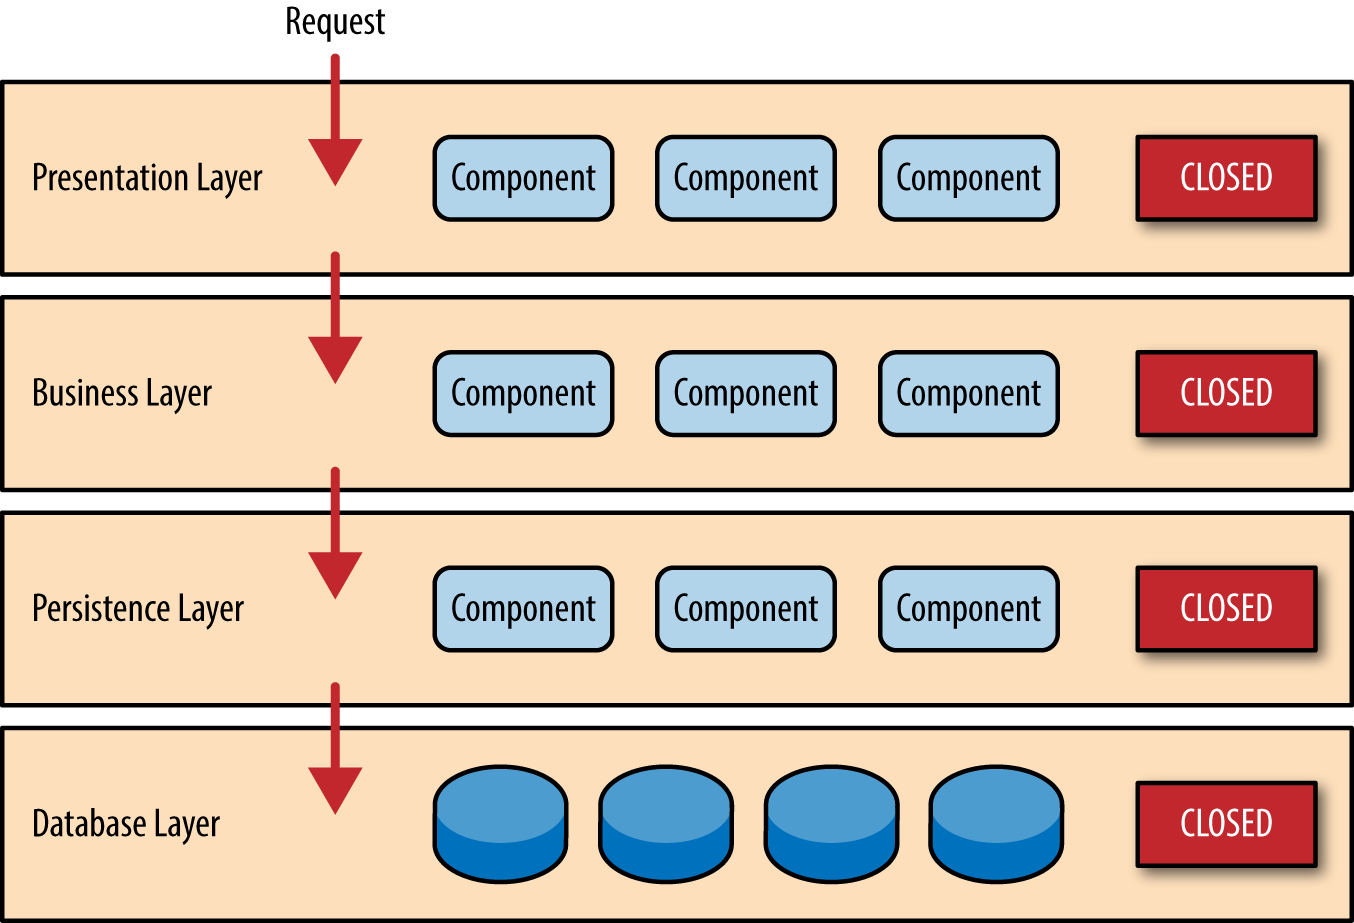
\includegraphics[height=6cm]{layered-architecture}
\end{figure}
\leavevmode\newline
Solitamente ogni livello comunica solo con il livello sottostante. Il connettore tra ogni livello può 
essere una chiamata di funzione, una richiesta di query, un oggetto dati o qualsiasi connettore che
trasmetta richieste o informazioni.
\\
La denominazione dei livelli è abbastanza flessibile ma di solito un livello di presentazione, un livello
di business e un livello fisico sono sempre presenti
\\\\
Livello di presentazione
\\
Il livello di presentazione contiene tutte le classi responsabili di presentare la visualizzazione delle
delle informazioni all'utente finale. Idealmente questo è il solo livello con cui l'utente finale 
interagisce.
\\\\
Livello di business
\\
Il livello di business contiene tutta la logica che è richiesta dall'applicazione per poter soddisfare i 
suoi requisiti funzionali. Solitamente questo livello si occupa dell'aggregazione dei dati, della computazione
e della richiesta dei dati. Quindi qui è dove viene implementata la logica principale dell'applicazione.
\\\\
Livello fisico
\\
Qui è dove sono salvati tutti i dati recuperabili dell'applicazione. Solitamente questo livello è chiamato
anche livello di persistenza. Questo livello si occupa di interagire con il sistema in cui i dati 
sono mantenuti in maniera persistente, come ad esempio un database.
\leavevmode\newline
\subsection{Motivazioni della scelta}
Le motivazione che hanno portato a scegliere questo stile architetturale sono le seguenti:
\begin{itemize}
    \item Dato che la separazione delle responsabilità è la proprietà principale di quest'architettura,
        ogni livello di software ha la sua specifica funzione. Questo rende facile il dover aggiornare 
        singoli livelli e permette al team di sviluppo di separare bene i carichi di lavoro tra i vari 
        membri, che possono lavorare in maniera contemporanea su livelli diversi.
    \item Per la proponente è importante avere una suite di test automatici per testare i vari componenti
        dell'applicazione. La layered architecture separando bene le responsabilità tra i livelli, 
        permette di suddividere l'applicazione in componenti ben separati e quindi più facili da testare.
        Essendo ogni livello isolato dagli altri, è possibile creare casi di test di dimensione ridotta, 
        in quanto le componenti di cui fare il mock sono poche.
    \item L'isolamento tra i vari livelli permette di modificare un livello senza che la modifica intacchi
        gli altri livelli.
    \item Nel caso l'applicazione diventi molto grande è possibile senza troppo sforzo avviare un processo
        di migrazione ad un'architettura a microservizi. La layered architecture lavora bene come monolite 
        in un sistema con un'architettura ibrida tra un monolite e un sistema a microservizi. Questa architettura
        ibrida andrà a formarsi nel mentre che il monolite viene migrato in un sistema a microservizi, quindi 
        è importante avere un architettura a monolite che lavori bene in questo tipo di sistema.
        \\
        Inoltre grazie alla separazione delle responsabilità della layered architecture è più facile andare
        a trasformare i componenti del monolite in microservizi.
\end{itemize}